%!TEX root = ../thesis.tex

\cleardoublepage
\chapter{Evaluation}
\label{cha:evaluation}

This chapter looks at the set-up for the experiments and presents and discusses the results achieved. In section \ref{sec:testing} the environment in which the agents were tested is explained and then in the section \ref{sec:analysis} the results are presented and discussed. 

\section{Testing the Agents}
\label{sec:testing}

In order to evaluate the performance of these agents they were tested on a 32-core, 125GB RAM machine against 5 different workflows from the popular bioinformatics framework nf-core \footnote{https://nf-co.re/}. Each workflow is first run 10 times without any reinforcement learning agents active. This was done to have something to compare the results to later but also so that there was historical data about the average execution time of each of the tasks, since the reinforcement learning agents need this information. After that the agents are tested. The gradient bandits are run 50 times for each workflow and the q-learning agent 100 times. As has been explained in \ref{subsub:states} the q-learning agent needs considerably longer to explore its extensive state-action space and as such needs to be trained for longer. However even though it is run twice as many times as the gradient bandit, the q-learning agent is still perhaps under-trained since the state-action space it needs to explore is so much larger than the action-space which the gradient bandit explores.

The five workflows used are the following: 1) \textit{eager} - a pipeline for genomic NGS sequencing data, 2) \textit{mhcquant} - a workflow for quantitative processing of data dependent (DDA) peptidomics data, 3) \textit{nanoseq} - which is an analysis pipeline for Nanopore DNA/RNA sequencing data, 4) \textit{viralrecon}- which can be  used to perform assembly and intra-host/low-frequency variant calling for viral sample, and 5)  \textit{metaboigniter} - a pipeline for pre-processing of mass spectrometry-based metabolomics data. 

The input data used for the workflows is based on custom combinations of different input files provided by the workflow's maintainers. Generally for each pipeline there are full example datasets and short example datasets as well as configurations for each of them. The short datasets are all configured to only assign either 1 or 2 CPUs and are thus are not really feasible for comparison, however the full datasets, whilst featuring realistic configurations, often take far too long to run. For reference, the full datasets will often take 6 hours or more to run once whereas the short examples never take more than 5 minutes. In order to build good pipelines with more realistic runtimes, configurations and input data, but without running too long, the short examples and the full ones need to be combined. The combinations are designed to strike a balance between having large input data and realistic task configurations but also being short enough that it is feasible to run the workflows hundreds of times. Each workflow’s set of inputs is built individually but the overarching tactic used was to start with the command line arguments to the pipeline from the short examples and combine those with the configuration and the input data from the full dataset. After this the list of input files is reduced until the pipeline completes in a reasonable amount of time. By following this process, configurations and inputs were found for all five of the pipelines mentioned above such that they were completing after around 10 to 40 minutes.  

Nextflow inherently keeps track of the total number of resources available and the resources already assigned to tasks and it will not schedule more resources than the system has left. The tasks are all run inside of docker containers with the exact amount of CPUs and memory requested by the task. Since the tasks are all being run on the same machine it would have been possible to ignore the sum of the resource requests and over-assign resources so that all of the tasks compete with each other, but this does not reflect situations where pipelines are being run on clusters with resource managers, and as such this was left unchanged.

For the final comparison in the next section the 10 runs with the default configurations are compared with the last 10 runs of each of the agents and 10 runs using a naive feedback loop approach. The naive approach functions as follows: first, during training, the workflows are run 10 times and each task is assigned the maximum number of CPUs and memory available. Then, in the next 10 runs the task are assigned the floor of the average number of CPUs used during the training and the mean amount of memory used plus the standard deviation. Should a task fail, then it is retried with the maximum amount of memory ever used by that task during the training time, and should it fail again then it is retried with double that value. This feedback loop approach has been mentioned in chapter \ref{cha:related_work} and it is loosely based on the work from \cite{tovarjob,FeedbackBasedAllocation}.



%%=========================================
\section{Results and Discussion}
\label{sec:analysis}

\subsection{Performance Comparison}
\label{sub:comp_perf}

\begin{figure}[h]
    \centering
        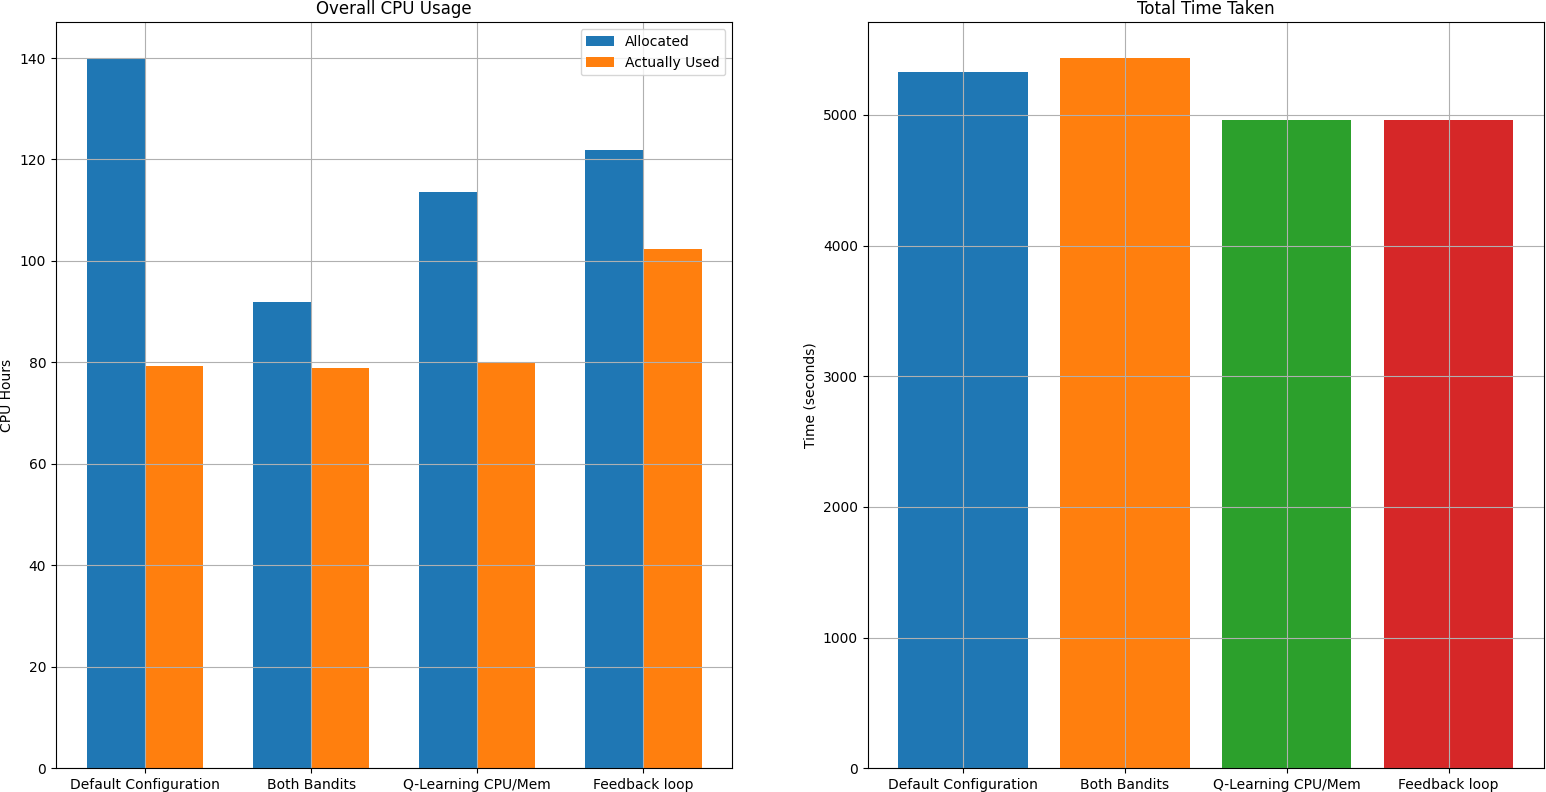
\includegraphics[width=\textwidth]{fig/cpu_mem_results.png}
        \caption{Performance of the CPU and Memory Approaches}
        \label{fig:cpu_results}
\end{figure}

\begin{figure}[ht]
    \centering
        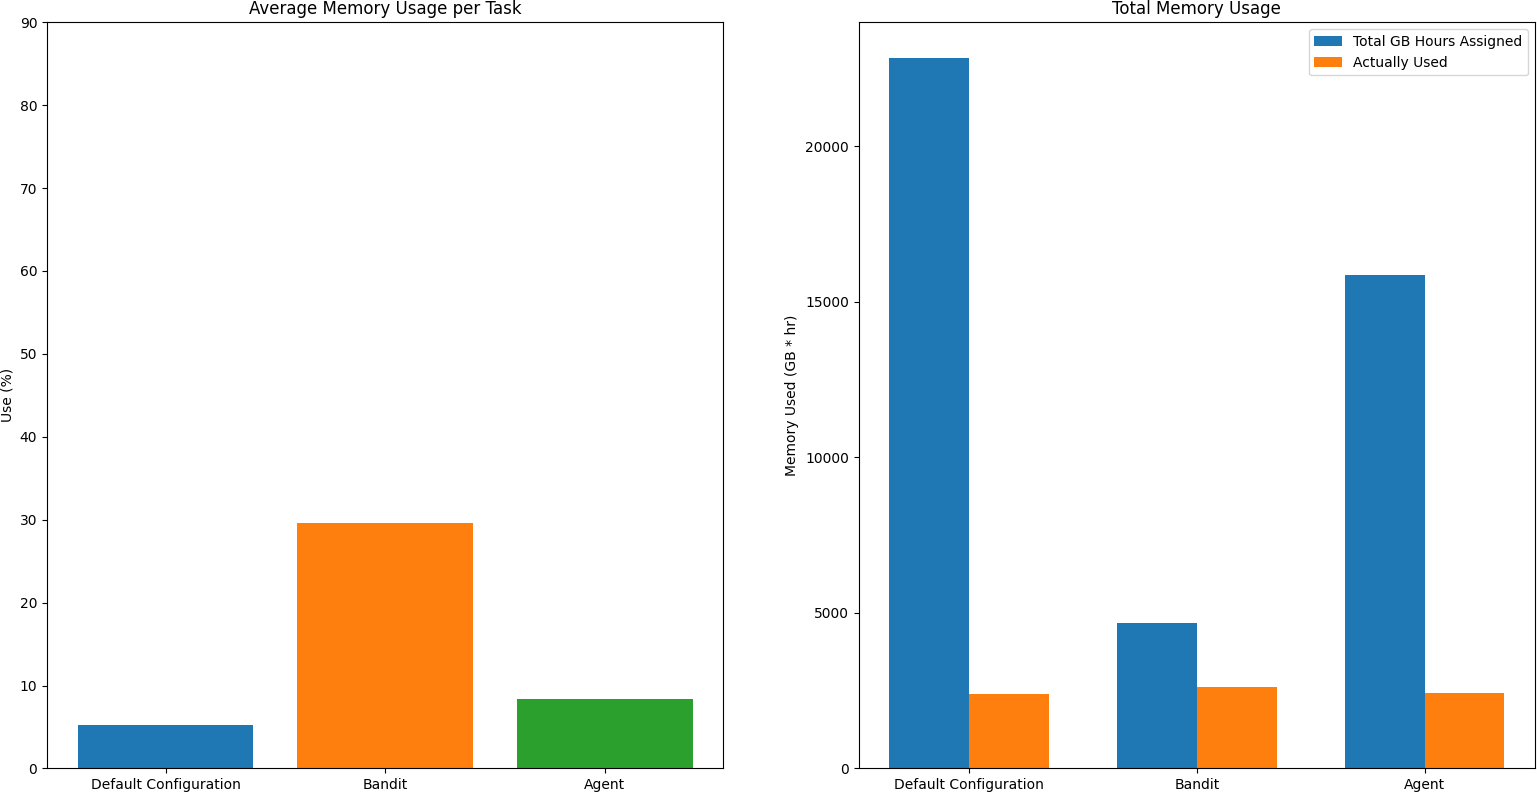
\includegraphics[width=\textwidth]{fig/cropped_memory_usage_final.png}
        \caption{Memory Usage}
        \label{fig:mem_use}
\end{figure}

In this section the performance of the gradient bandit and the q-learning approaches over their last 10 runs will be compared with each other and with the performance of the default configuration and the naive approach using a feedback loop.

The figures \ref{fig:cpu_results} and \ref{fig:mem_use} show the performance of all of these approaches. The left graph in the first figure shows the total amount of CPU hours requested by all of the tasks across all of the workflows and the amount of CPU hours that were effectively used (calculated as $cpu\_usage/100*time$ and $cpus*time$ respectively). The right graph in this figure shows the total time it took for all of the workflows to complete. Additionally in \ref{fig:mem_use}, the memory usage is shown. The unit measured in the right graph is the gigabyte hour and the graph displays the total amount of gigabyte hours allocated across all of the workflows as well as the actual amount of gigabyte hours used (based on each task’s peak RSS and execution time- this is the minimum amount of gigabyte hours which could have been assigned without the task being killed). The left graph shows the average memory usage of each individual task (calculated as $\frac{peak\_rss}{memory}$). 

From these graphics it is clear to see that all of the reinforcement learning approaches managed to improve CPU efficiency and allocate less CPU hours than both the default configuration and the naive feedback loop approach. In the case of the gradient bandit it was particularly effective at keeping the overall CPU hours assigned to an absolute minimum, however it seems that this efficiency came at the cost of speed, and it performed worse than its q-learning counterpart in this aspect, and took slightly longer than the default configuration. The q-learning approach took almost exactly the same amount of time as the feedback loop but was more efficient with regards to CPU usage. As can be seen, both of the reinforcement learning approaches are able to assign less CPU hours without having a detrimental effect on execution time (in fact the q-learning approach assigns less CPU hours but executes faster). Looking at the reward function \ref{q_agent_1_reward} for the q-learning agent the “CPU usage”considered by the function is not the task’s usage of the task but rather $max(90,CPU\_usage)$. As such agents for tasks which exhibit very high CPU usage ($>90\%$) receive no additional reward for increased efficiency (since efficiency can always be increased by decreasing the total number of CPUs assigned) so their rewards depend entirely on the execution time and they are thus encouraged to find resource allocations which decrease runtime. This most likely explains why the gradient bandit is more efficient but the q-learning agent is faster.

Interestingly, the feedback loop ultimately wound up increasing the effective CPU hours used by the workflows, something which had remained constant under the other 3 configurations, and the naive approach was fairly efficient in terms of the total amount of CPU hours assigned- relative to the increased effective usage. It can only be speculated as to why it used more actual CPU hours than the other approaches but it may be down to the fact that certain highly parallelizable tasks will be assigned incredibly large numbers of CPUs (e.g. a task with 2800\% CPU usage during training will be assigned 28 CPUs) far beyond the point of diminishing returns, and eventually lead to the workflow using more effective CPU hours. This would indicate that assigning more resources may increase the amount actually used which the feedback loop approach assumes is false.

Finally, regarding execution time, it is interesting to see that the q-learning approach is able to match the performance of the feedback loop despite assigning less CPU hours overall. In this regard the q-learning approach could be considered optimal relative to the other approaches. The gradient bandit ultimately over-emphasized decreasing costs and performed worse whilst the feedback loop approach over-emphasized attempting to increase performance by increasing CPU usage and wound up using more resources than would have been necessary to achieve the same execution time. The q-learning agent was able to find the best balance between resource usage and performance. This is of course the benefit of a reinforcement learning approach- it can estimate the values of a complex reward function by exploring different actions and then pick the maximizing action. The feedback loop approach cannot explore different allocations on its own and is dependent on the correctness of its assumptions and the quality of its input data.

Concerning memory allocations, both of the reinforcement learning approaches proved to be better than the default configuration. One aspect which stands out is how poor the default configurations are. Indeed on average they are using just 5\% of the assigned memory on a task by task basis . On the other hand the q-learning approach is not much more efficient, however it still reduces the wasted memory by a large amount (~5000 gigabyte hours saved compared to the default configuration). Yet this amount is dwarfed by the other two approaches which save close to 15000 gigabyte hours. The memory bandit approach performed better than the q-learning approach by a significant margin and it assigned less than half as much as either the default configuration or the q-learning agent. The feedback loop approach is clearly the best, assigning the least amount of memory hours overall and showing very high memory usage for all of the tasks.

Ultimately the performance of the q-learning agent is down to the fact that the number of chunks of memory it could choose from was very low (in order to have less states so it could be trained faster), and thus it had a fairly limited extent to which it could reduce the memory usage. The gradient bandit suffers from this too because ultimately it also only had a fixed number of memory chunks to choose from and could only increase or decrease a task’s memory usage by a multiple of the size of the memory chunk. The feedback loop does not have this problem and can assign memory at the most granular level possible. It therefore follows that it would naturally be able to outperform these two approaches which can only assign “discrete” chunks of memory. Another factor to consider is that both of the reinforcement learning approaches also had the option to assign more memory than the default configuration. This was clearly unnecessary and because all of the tasks were using much less memory than the default amount it would have been possible to change the agents options to only be chunks of memory which added up to less than the default amount. This would have increased their performance. 


\subsection{Summary}
\label{sub:summary}

In conclusion all of the reinforcement learning approaches were able to intelligently size the tasks in the workflows and in the end the overall number of CPU hours which were wasted was reduced relative to both the feedback loop and the default configurations. In addition to this the agents were also able to significantly reduce the memory usage compared to the default configuration but struggled to reach the near-optimal performance of the feedback loop. The gradient bandit took slightly longer on average but was much more efficient for that, whilst the q-learning agent struck a better balance between resource efficiency and increased performance and the q-learning approach was ultimately able to outperform the default configurations in both resource efficiency and runtime.

While it could be argued that the q-learning agent is therefore the “better” option it is hard to say exactly what the right approach is because it also depends on the desires of the user. Many scientists may be prepared to accept slightly longer runtimes if the “greediness” of their workflows is decreased and they are able to free up resources for others to use, or reduce their own costs (if they are paying for CPU hours). Indeed from a financial perspective the gradient bandit wastes significantly less CPU hours than the extra time it takes to complete, which is fairly marginal. However in a situation where the user is paying for the entire system and not for resource usage it may make more sense from a financial perspective to use the q-learning agent approach since it reduces the amount of time for which the system needs to be up by reducing the overall execution time. Finally, it should be pointed out that combining the feedback loop’s memory approach and a q-learning agent which only considers CPU assignments would yield the best overall performance.
